% License: CC BY-SA
% Authors: See authors below and see also acknowledgement for authors of some images or research

% EGU: http://meetingorganizer.copernicus.org/EGU2015/posters/17174
%      http://meetingorganizer.copernicus.org/EGU2015/EGU2015-8314-7.pdf

\documentclass[25pt, margin=0mm, innermargin=15mm, blockverticalspace=15mm, colspace=15mm, subcolspace=8mm]{tikzposter}
\geometry{paperwidth=197cm,paperheight=100cm}

% to stretch boxes over whole paper with custor paper size
\makeatletter
\setlength{\TP@visibletextwidth}{\textwidth-2\TP@innermargin}
\setlength{\TP@visibletextheight}{\textheight-2\TP@innermargin}
\makeatother


\usepackage[utf8]{inputenc}
\usepackage{wrapfig}
\usepackage[hidelinks]{hyperref}

% For bibliography styling
%% TODO: all names should be abbreviated
\usepackage{natbib}

\definecolor{titleTextColor}{HTML}{009000}
\definecolorpalette{grassColorPalette} {
  \definecolor{colorOne}{HTML}{419041}
}
\usecolorstyle[colorPalette=grassColorPalette]{Britain}

\title{
\Huge
\textcolor{titleTextColor}{
\textsf{\textbf{
\fontsize{85}{60}\selectfont
GRASS GIS: a peer-reviewed scientific platform and future research repository
}}
}
}

\newlength{\grasslogoheight}
\setlength{\grasslogoheight}{0.08\textheight}
\newlength{\instlogoheight}
\setlength{\instlogoheight}{0.35\grasslogoheight}

\titlegraphic{
\begin{minipage}{0.3\linewidth}

\includegraphics[height=\grasslogoheight]{grass}
~

\includegraphics[height=\grasslogoheight]{osgeo_project}
\end{minipage}
\hfill
\begin{minipage}{0.2\linewidth}
\setlength{\baselineskip}{120pt}
\begin{flushright}

\includegraphics[height=\instlogoheight]{iwmi}
~

\includegraphics[height=\instlogoheight]{ncstate}
~

\includegraphics[height=\instlogoheight]{ctu_prague}
~

\includegraphics[height=\instlogoheight]{ti}
~

\includegraphics[height=\instlogoheight]{eurac}
~

\includegraphics[height=\instlogoheight]{fem_cri}
~

\includegraphics[height=\instlogoheight]{ec_jrc}
~

\includegraphics[height=\instlogoheight]{tib}
\end{flushright}
\end{minipage}
\vspace{-\grasslogoheight}
}

% \setlength{\blocktitleheight}{0.02\textheight}

% style for institute numbers
\newcommand{\inst}[1]{\hspace{2pt}$^{\mbox{\normalsize#1}}$\hspace{-7pt}}
\newcommand{\instlist}[1]{\hspace{1pt}$^{\mbox{\normalsize#1}}$\hspace{2pt}}

\author{
Yann Chemin\inst{1},
V\'{a}clav Petr\'{a}\v{s}\inst{2},
Anna Petr\'{a}\v{s}ov\'{a}\inst{2},
Martin Landa\inst{3},
S\"{o}ren Gebbert\inst{4},
Pietro Zambelli\inst{5},
Markus Neteler\inst{6},
Peter L\"{o}we\inst{7}, and
Margherita Di Leo\inst{8}
}
\institute{
\instlist{1}IWMI, Sri Lanka;
\instlist{2}NCSU, USA;
\instlist{3}FCE CTU in Prague, Czech Republic;
\instlist{4}TICSA, Germany;
\instlist{5}EURAC, Italy;
\instlist{6}CRI, FEM, Italy;
\instlist{7}TIB Hannover, Germany;
\instlist{8}EC-JRC, Italy
}

\hypersetup
{
    pdfauthor={Y. Chemin, V. Petras, A. Petrasova, M. Landa, S. Gebbert, P. Zambelli, M. Neteler, P. Loewe, M. Di Leo},
    pdfsubject={},
    pdftitle={GRASS GIS: a peer-reviewed scientific platform and future research repository},
    pdfkeywords={GIS, algorithms, methods, preservation, science, reproducibility}
}

% \usetemplate{1}
% \setinstituteshift{1}

% \setblocktitleheight{2}
% \setblockspacing{1}

\graphicspath{{images/}{logos/}}

\newcommand{\blocktitlewrap}[1]{\textsf{\textbf{\huge#1}}}
% it is not possible (?) to change block title in the class, using wrapper
% the command introduced using:
%   sed -i 's/\\block{\([^}]*\)}/\\block{\\blocktitlewrap{\1}}/g' main.tex

% GRASS module
\newcommand{\gmodule}[1]{\href{http://grass.osgeo.org/grass70/manuals/#1.html}{\emph{#1}}}
\newcommand{\gamodule}[1]{\href{http://grass.osgeo.org/grass70/manuals/addons/#1.html}{\emph{#1}}}
\newcommand{\gmodulenolink}[1]{\emph{#1}}

\begin{document}
\maketitle[width=0.92\textwidth]
% \maketitle
% \addlogo[north west]{(2,-1)}{9cm}{images/Grass_GIS}
%Please insert your institution logo here
% \addlogo[north east]{(-2,-2.5)}{4cm}{images/logo_FEM_CRI}
% \addlogo[north east]{(-2,-5.5)}{4cm}{images/NC_State_Seal}
% \addlogo[north east]{(-8,-2.5)}{4cm}{images/Logo_cvut}
% \addlogo[north east]{(-8,-6.5)}{4cm}{images/IWMI_logo}
% \addlogo[north east]{(-2,-10.5)}{4cm}{images/logo_ec-jrc}

\begin{columns}

%%%%%%%%%%%%%%%%%%%%%%%%%%%%%%%%%%%%%%%%%%%%%%%%%%%%%%%%%%%%%%%%%%%%%
%%%%%%%%%%%%%%%%%%%%%%%%%%%%%%%%%%%%%%%%%%%%%%%%%%%%%%%%%%%%%%%%%%%%%
%%%%%%%%%%%%%%%%%%%%%%%%%%%%%%%%%%%%%%%%%%%%%%%%%%%%%%%%%%%%%%%%%%%%%
%%%%%%%%%%%%%%%%%%%%%%%%%%%%%%%%%%%%%%%%%%%%%%%%%%%%%%%%%%%%%%%%%%%%%
\column{0.25}

%%%%%%%%%%%%%%%%%%%%%%%%%%%%%%%%%%%%%%%%%%%%%%%%%%%%%%%%%%%%%%%%%%%%%%%%%%%%%%%%
\block{\blocktitlewrap{Introduction}}
{
\setlength{\parskip}{0.3ex}

Over the last decades, GIS has become a key driver in geospatial science, research and application.
GIS software which is licensed under a free and open source software (FOSS) licence
is more than just a mere tool for spatial analysis.

GRASS GIS (Neteler et al., 2012 \cite{neteler2012grass}), a free and open source GIS,
is used by many scientists directly or as a backend in other projects
such as R or QGIS to perform geoprocessing tasks.

Thanks to the user and developer community, submitted code is evaluated
in different fields of application beyond
the field of expertise of the original authors, and different scales of magnitude
of data.
This exceeds the established review process for scientific writing in a given journal
or a data publication in a defined field of science.

Immediate access to the software repository enables instant quality checking
of the current software version both by continuous automated tests (Petras, 2014 \cite{Petras2014}),
and code review by human experts.

New scientific algorithms can be developed against the reviewed functionalities
already provided by the GRASS GIS codebase.
This avoids unnecessary overheads, by re-implementation,
ensures quality by use of trusted components and allows reuse and long term preservation
within the project software repository.
Integrating scientific algorithms into GRASS GIS helps to preserve reproducibility
of scientific results over time as the original author designed it
(Rocchini \& Neteler, 2012 \cite{rocchini2012let}).
}

%%%%%%%%%%%%%%%%%%%%%%%%%%%%%%%%%%%%%%%%%%%%%%%%%%%%%%%%%%%%%%%%%%%%%%%%%%%%%%%%
\block{\blocktitlewrap{Landform detection: Geomorphons}}{

Jasiewicz and Stepinski \cite{jasiewicz2013geomorphons} developed a method and module \gamodule{r.geomorphon}
which provide orientation-invariant and relief-invariant method to classify landforms
in a scale-independent way.
Ashtekar et al. \cite{ashtekar2014digital} used geomorphons to study soil properties in northwestern South America.

\bigskip
\begin{minipage}{0.5\linewidth}
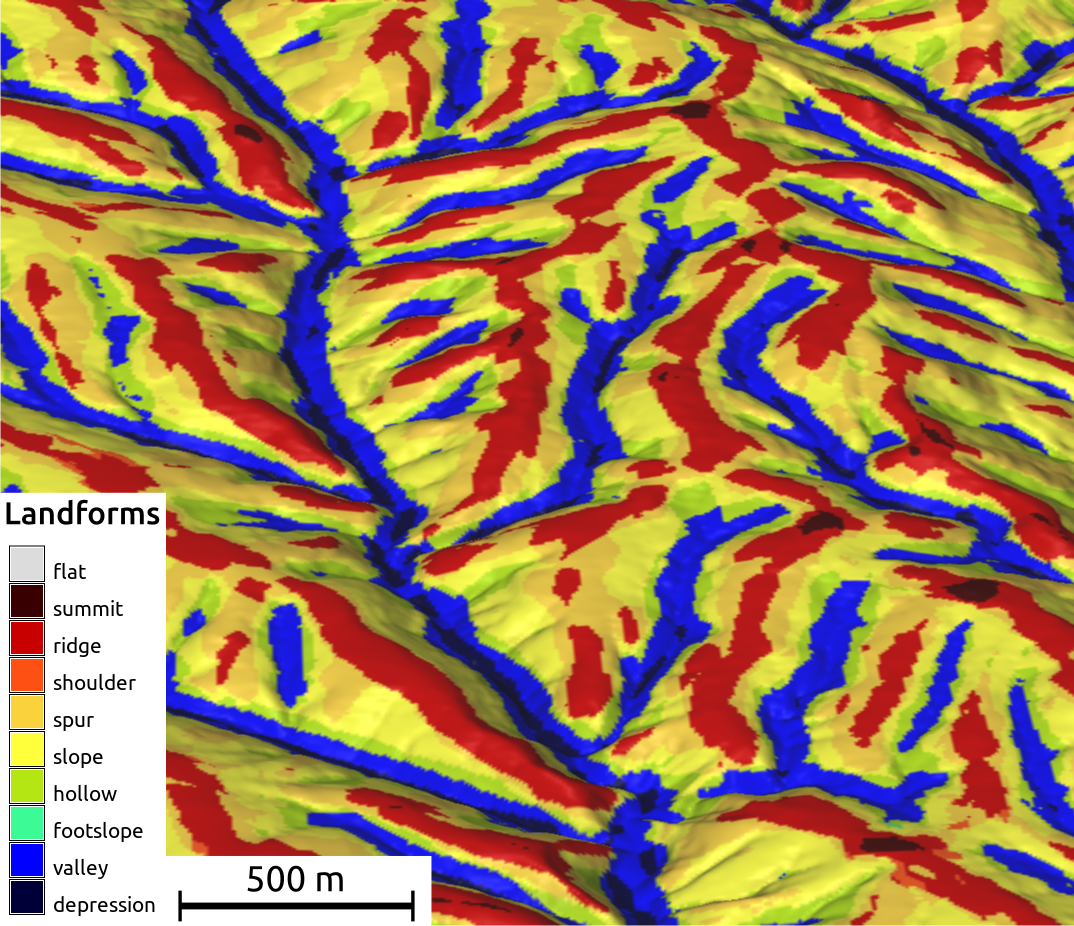
\includegraphics[width=\textwidth, trim={0 0 0 185}, clip]{geomorphon}
Geomorphons for part of Yakima Training Center (area 5x3~km, USA)
\end{minipage}
~
\begin{minipage}{0.5\linewidth}
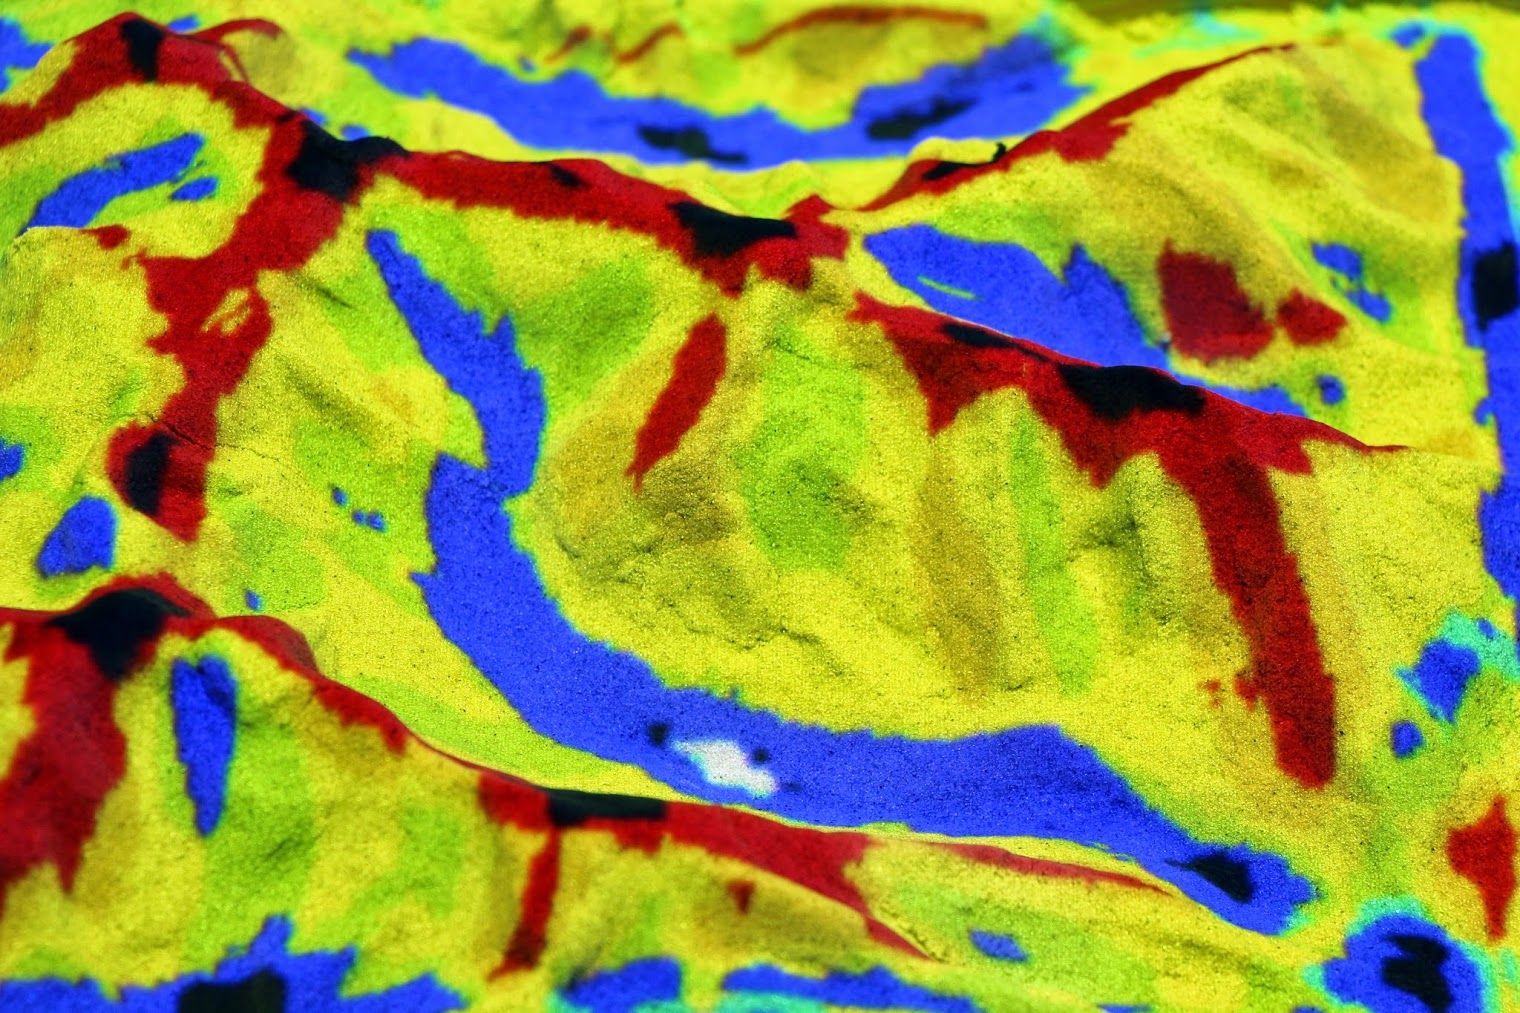
\includegraphics[width=\textwidth, trim={0 30 0 90}, clip]{geomorphon_tangible_high_tatras}
Ridges and valleys detected on the sand physical model of High Tatras (Slovakia) using \gamodule{r.geomorphon} integrated in Tangible Landscape system
\end{minipage}
}


%%%%%%%%%%%%%%%%%%%%%%%%%%%%%%%%%%%%%%%%%%%%%%%%%%%%%%%%%%%%%%%%%%%%%%%%%%%%%%%%
\block{\blocktitlewrap{Natural Hazards: Wildfire Spread}}{
The wildfire simulation toolset, originally developed by Xu (1994~\cite{xu1994simulating}) 
implements Rothermel’s model~\cite{Rothermel1983how}. It is available through the GRASS GIS 
modules \gmodule{r.ros} and \gmodule{r.spread} and is object of active research. It has been extensively 
tested and recently adapted to European fuel types (Rodriguez-Aseretto et al.,
2013~\cite{rodriguez2013data}; de Rigo et al., 2013~\cite{derigo2013architecture};
Di Leo et al., 2013~\cite{2013_DiLeo_etAl}).

\vspace*{-1cm}

\begin{minipage}{0.5\linewidth}
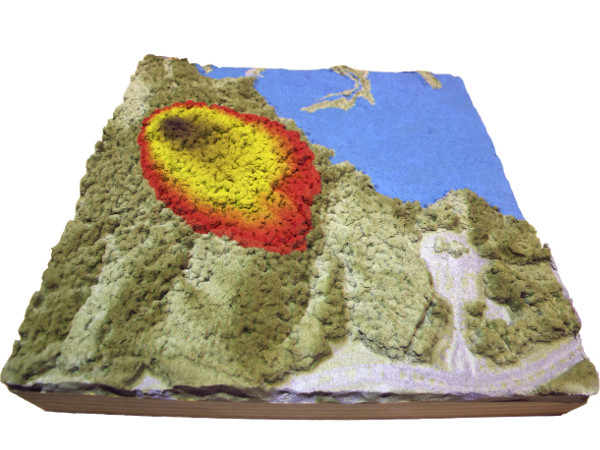
\includegraphics[width=\textwidth]{fire}
Wildfire simulation in Tangible Landscape environment
\end{minipage}
~
\begin{minipage}{0.5\linewidth}
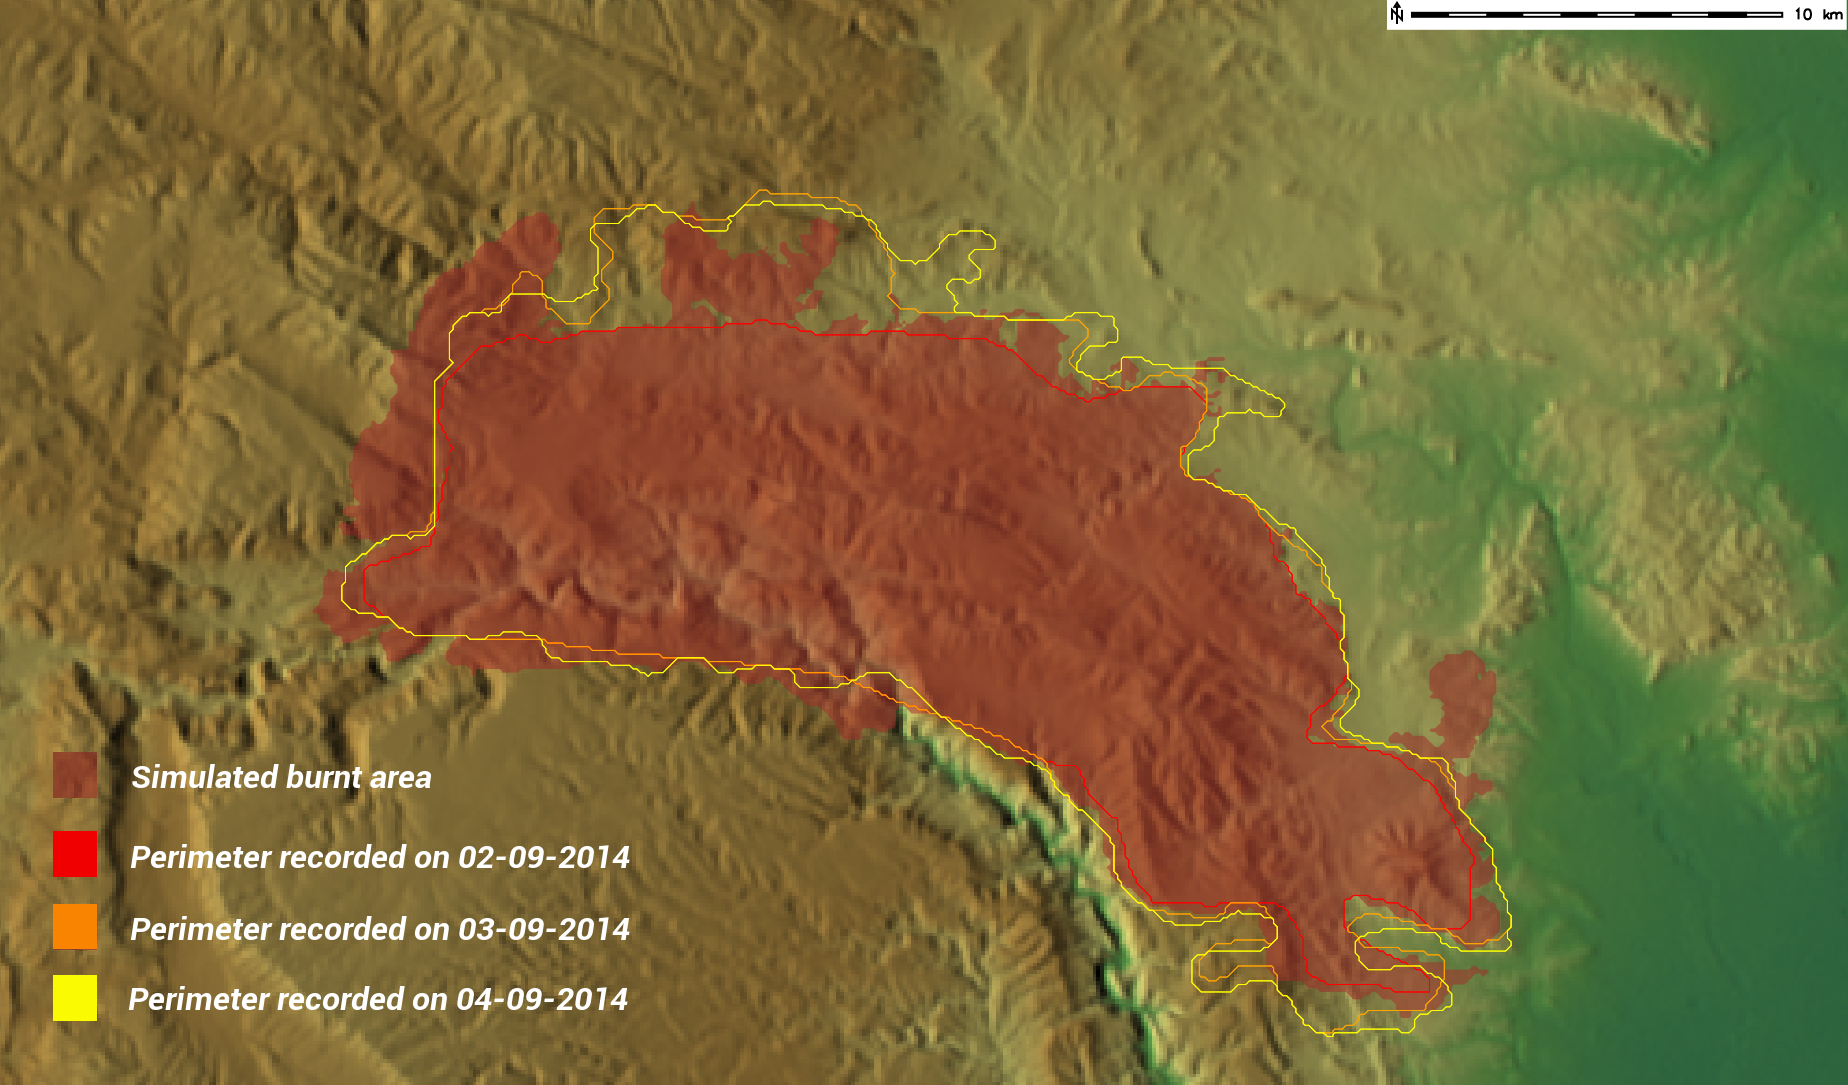
\includegraphics[width=\textwidth]{fire_valencia_040914}
Major wildfire event near Valencia (Spain) between June 28th and July 4th 2012.
The actual perimeters recorded by JRC-EFFIS are shown, in 
comparison with burnt area simulated in GRASS GIS.
\end{minipage}
}

%%%%%%%%%%%%%%%%%%%%%%%%%%%%%%%%%%%%%%%%%%%%%%%%%%%%%%%%%%%%%%%%%%%%%
%%%%%%%%%%%%%%%%%%%%%%%%%%%%%%%%%%%%%%%%%%%%%%%%%%%%%%%%%%%%%%%%%%%%%
%%%%%%%%%%%%%%%%%%%%%%%%%%%%%%%%%%%%%%%%%%%%%%%%%%%%%%%%%%%%%%%%%%%%%
%%%%%%%%%%%%%%%%%%%%%%%%%%%%%%%%%%%%%%%%%%%%%%%%%%%%%%%%%%%%%%%%%%%%%
\column{0.25}

%%%%%%%%%%%%%%%%%%%%%%%%%%%%%%%%%%%%%%%%%%%%%%%%%%%%%%%%%%%%%%%%%%%%%
\block{\blocktitlewrap{GRASS GIS as Temporal GIS}}{
The time dimension was introduced in GRASS GIS version 7 for raster, 3D raster and
vector map layers, transforming it into a full featured temporal GIS (Gebbert and Pebesma, 2014 \cite{Gebbert20141}).
Time series of map layers are managed in space time datasets, a new data type in GRASS GIS.
Based on the GRASS GIS Temporal Framework, more than 45 modules were implemented to manage, analyze, process
and visualize space time datasets. The temporal enabled GRASS GIS is capable of efficiently
handling more than 100,000 map layers; e.g., it was used to analyze the
European Climate Assessment \& Dataset ECA\&D (Haylock et al. \cite{Haylock2008_climate_series})
for climate change indicators.

\vspace*{1cm}

\begin{minipage}{0.5\linewidth}
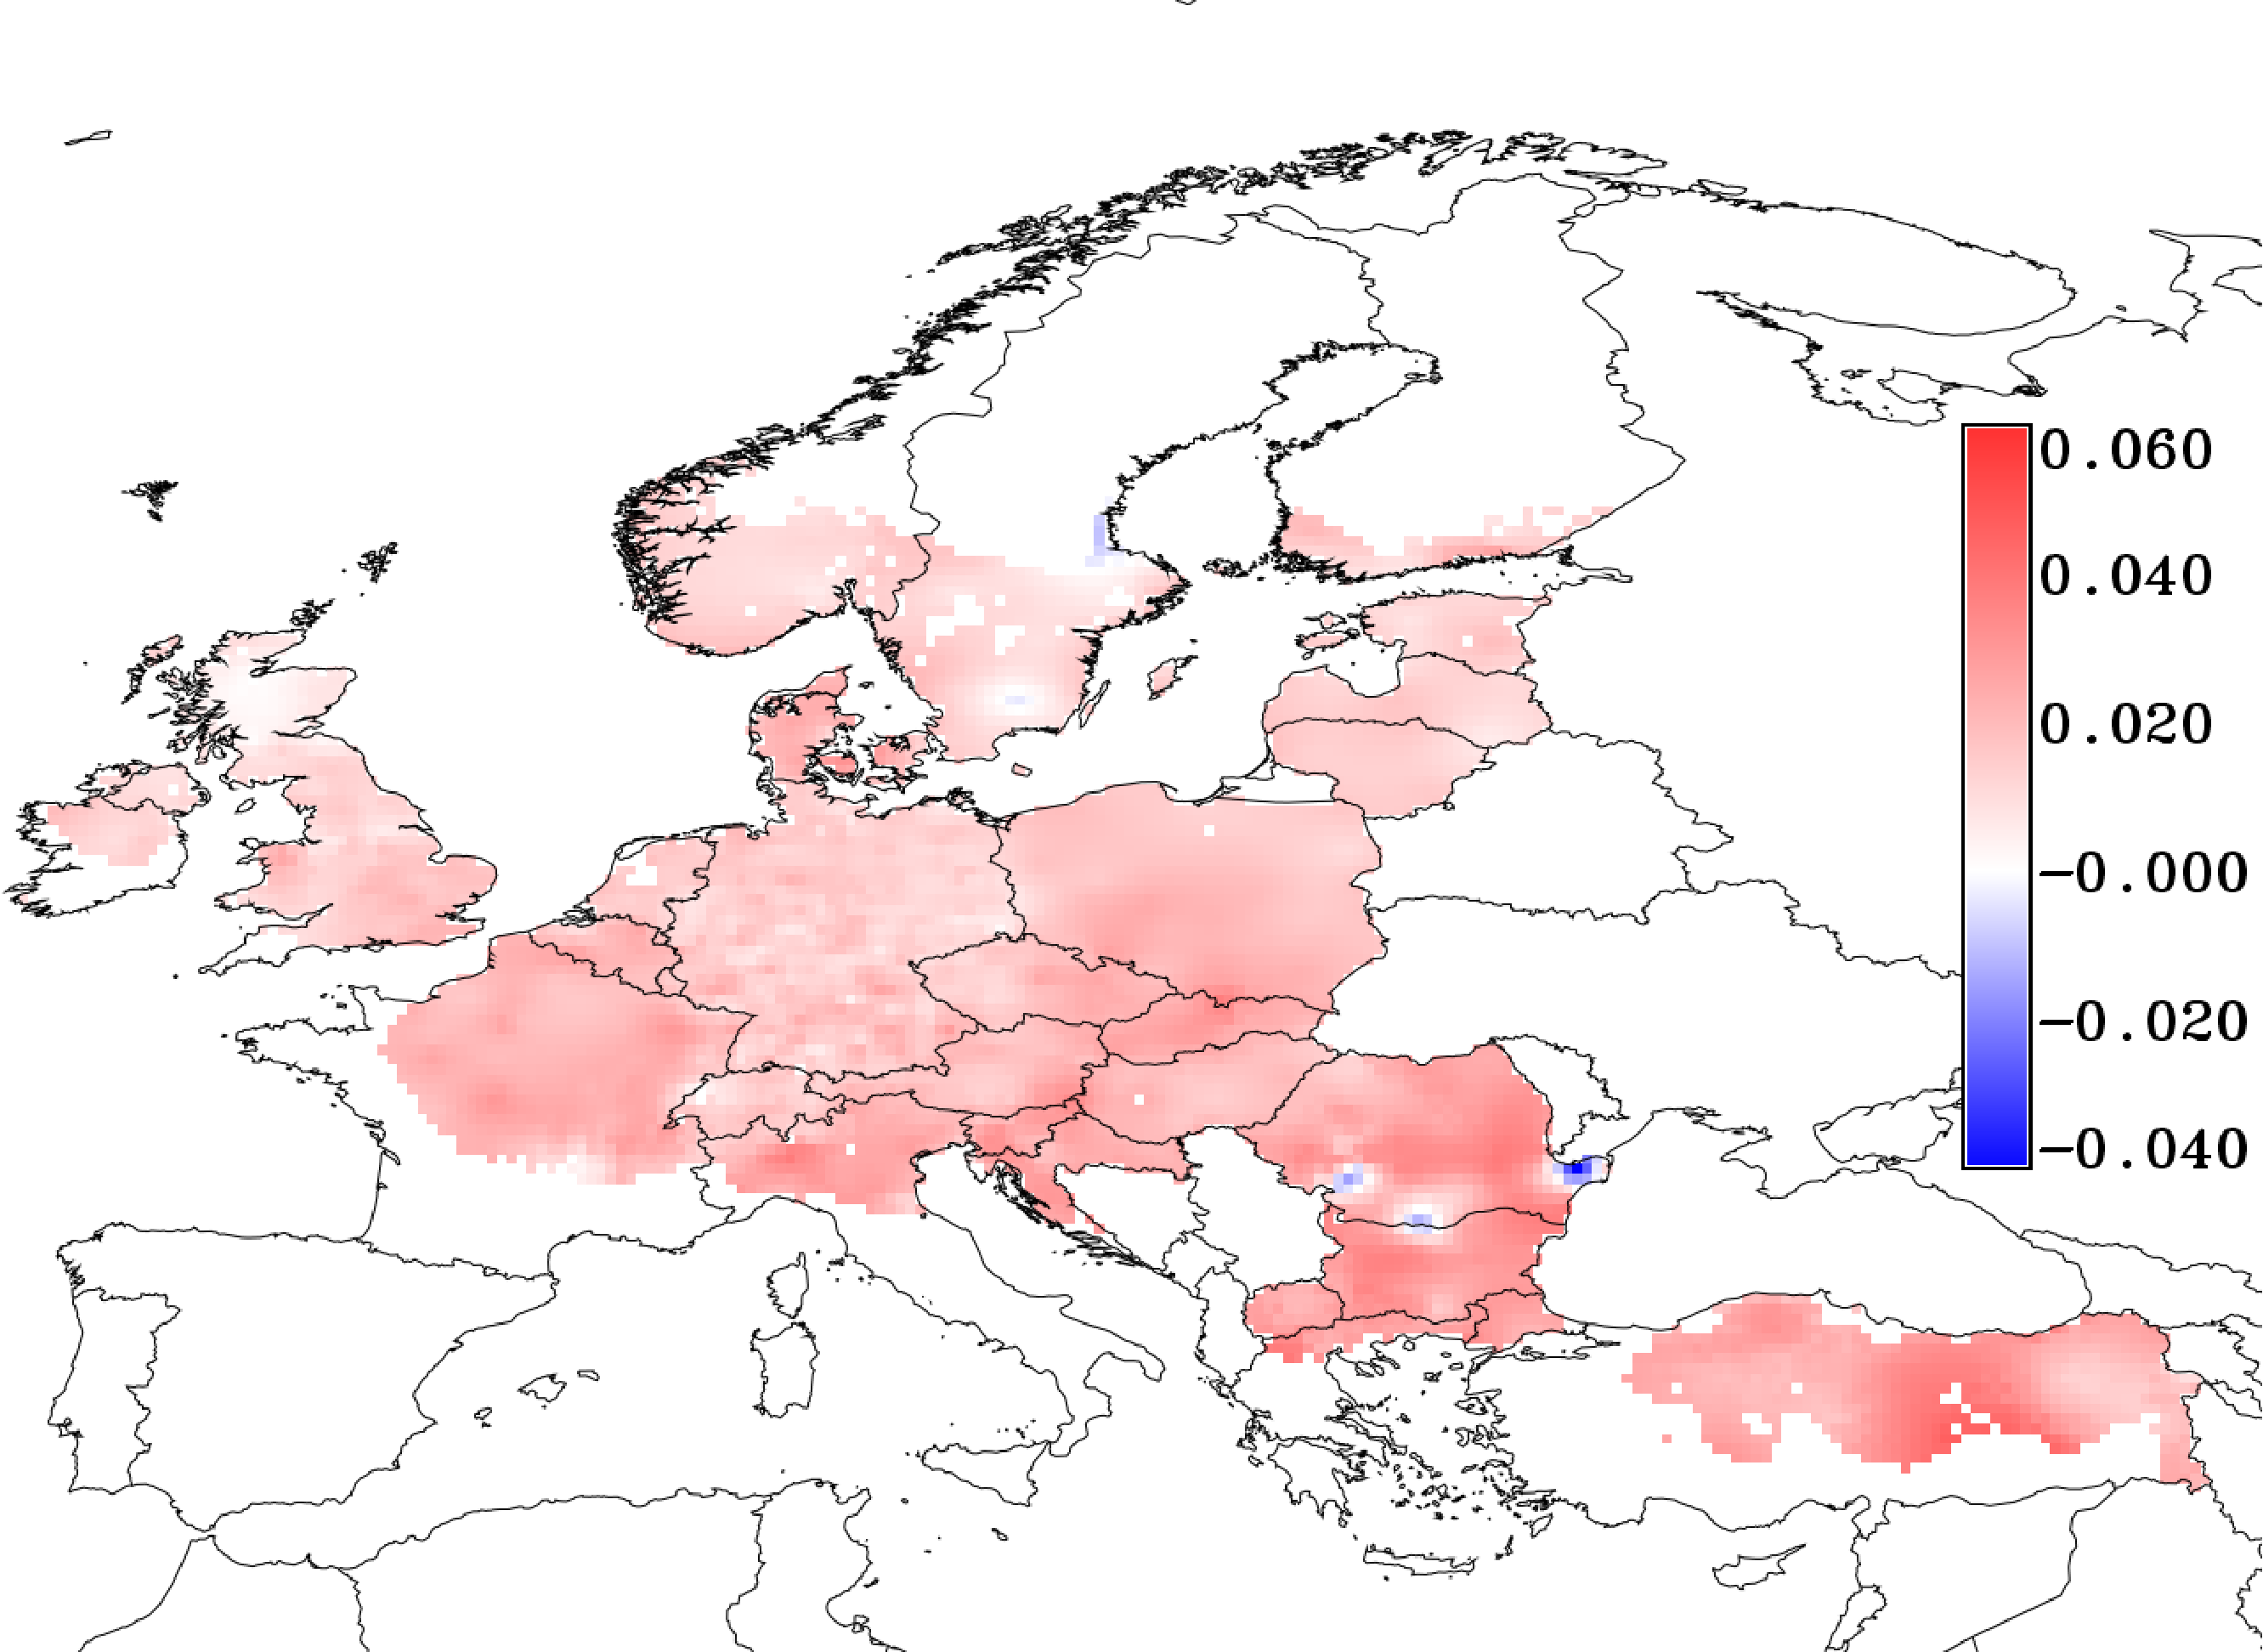
\includegraphics[scale=0.5]{images/summer_mean_temp_slope.pdf}
The linear regression slope computed with t.rast.series of the temperate climate zone in the European Union
for summer season from 1950 - 2011 (Gebbert and Pebesma, 2014 \cite{Gebbert20141}). Red color
indicates rising temperature, blue indicates falling temperature. Units are degree Celsius per year.
\end{minipage}
~
\begin{minipage}{0.5\linewidth}
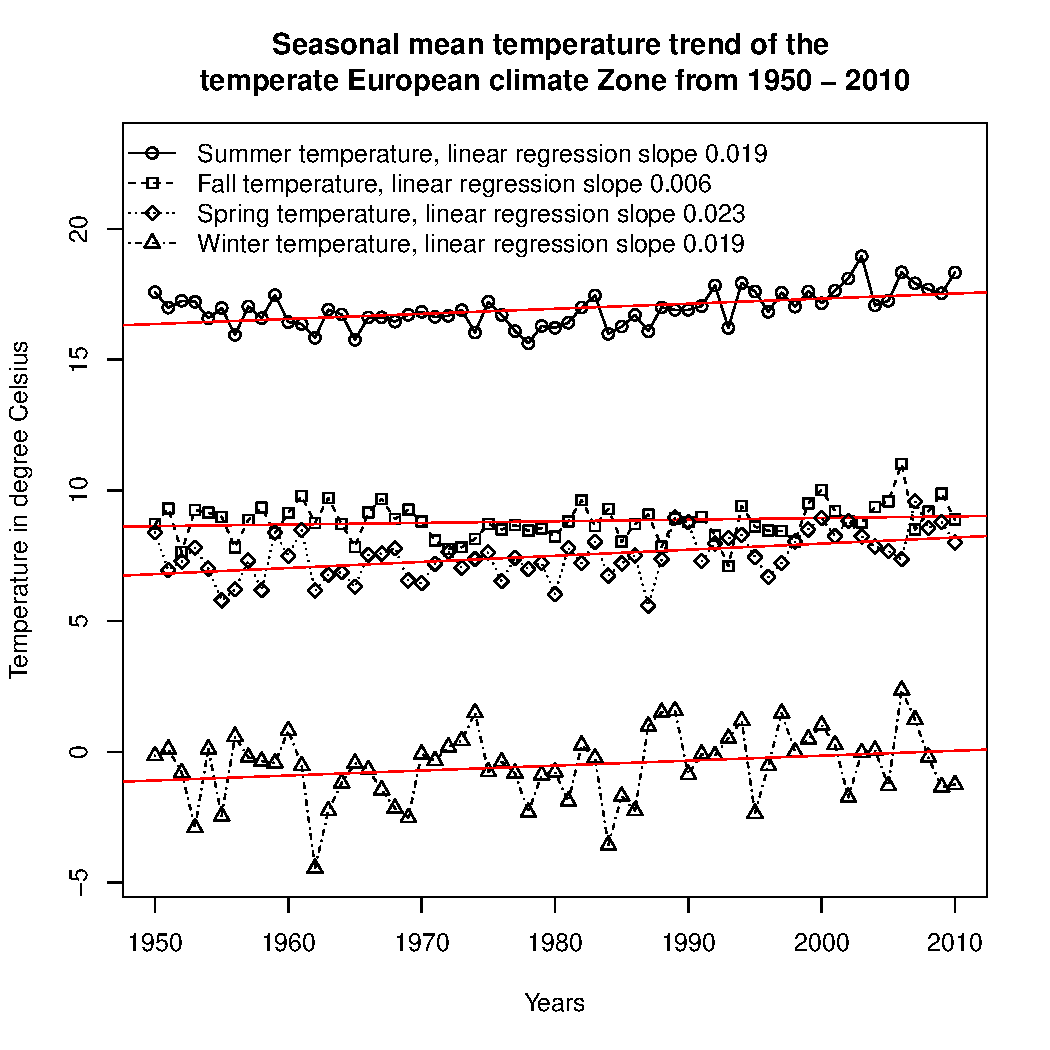
\includegraphics[scale=1.25]{images/Seasonal_temperature_trend_Europe_1950_2010.pdf}
Seasonal mean temperature trend for the temperate climate zone of the European Union
(Gebbert and Pebesma, 2014 \cite{Gebbert20141}). The modules \gmodule{t.rast.aggregate},
\gmodule{t.rast.univar} and the open source statistical software system R
were used to create this plot.
\end{minipage}

\vspace*{1cm}

}


%%%%%%%%%%%%%%%%%%%%%%%%%%%%%%%%%%%%%%%%%%%%%%%%%%%%%%%%%%%%%%%%%%%%%
%%%%%%%%%%%%%%%%%%%%%%%%%%%%%%%%%%%%%%%%%%%%%%%%%%%%%%%%%%%%%%%%%%%%%%%%%%%%%%%%%
\block{\blocktitlewrap{Natural Hazards: Water, Floods and Erosion}}{

GRASS GIS entails several modules that constitute the result of active research on natural hazards.
The \gmodule{r.sim.water} simulation model (Mitas and Mitasova, 1998 \cite{Mitas1998b})
for overland flow with spatially variable rainfall excess conditions was integrated into the Emergency
Routing Decision Planning system as a WPS (Raghavan et al., 2014 \cite{raghavan2014deploying}).
The module \gmodule{r.sim.water} together with
the module \gmodule{r.sim.sediment} for erosion-deposition modeling
implements a path sampling algorithm which is robust and easy to parallelize.
The \gmodule{r.sim.water} module was also utilized by Petrasova et al., 2014 \cite{Petrasova2014} and is now part of
\emph{Tangible Landscape}, a tangible GIS system, which also incorporated \gmodule{r.damflood},
a dam break inundation simulation \cite{cannata2012two}.

\bigskip

\vspace*{1cm}

\begin{minipage}{0.5\linewidth}
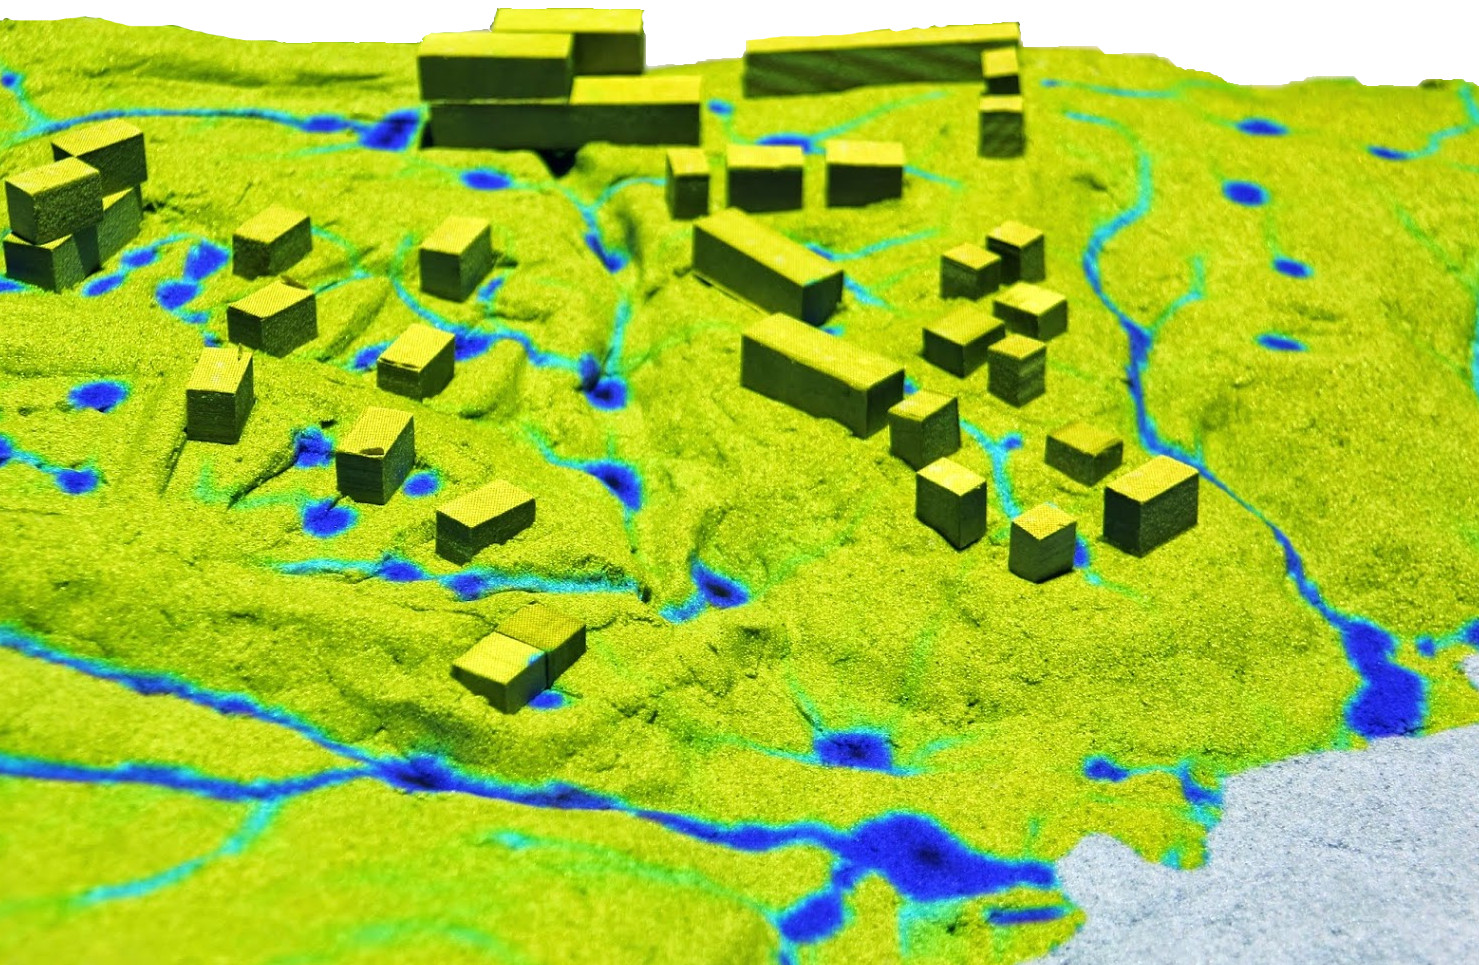
\includegraphics[width=\textwidth]{rsimwater_architects}
Overland flow used for landscape architecture design in Tangible Landscape environment
\end{minipage}
~
\begin{minipage}{0.5\linewidth}
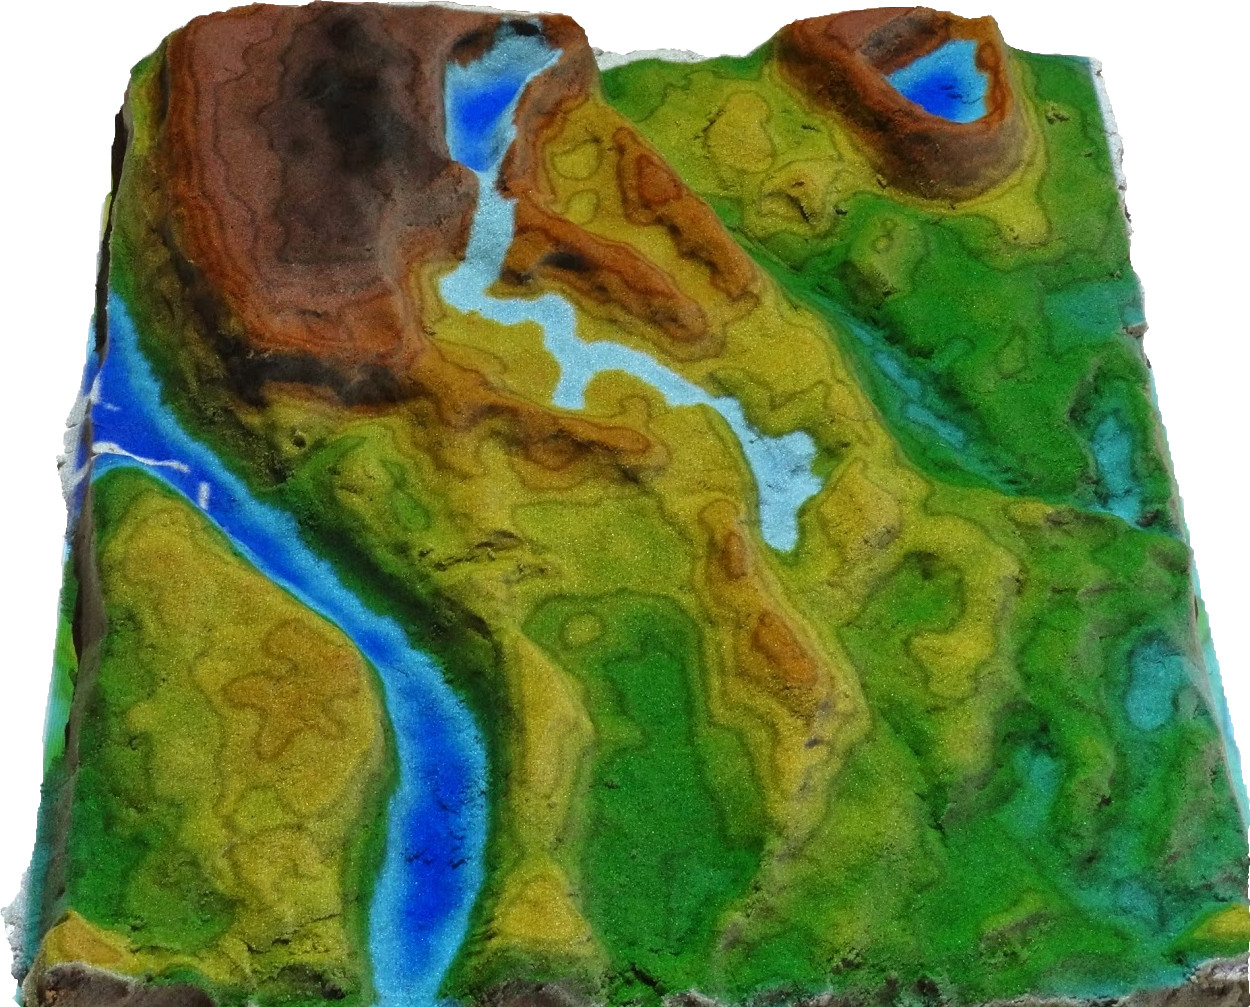
\includegraphics[width=\textwidth]{damflood_tangible}
Coal ash pond breach in Tangible Landscape environment using \gamodule{r.damflood} module
\end{minipage}

\vspace*{1.4cm}
}


%%%%%%%%%%%%%%%%%%%%%%%%%%%%%%%%%%%%%%%%%%%%%%%%%%%%%%%%%%%%%%%%%%%%
%%%%%%%%%%%%%%%%%%%%%%%%%%%%%%%%%%%%%%%%%%%%%%%%%%%%%%%%%%%%%%%%%%%%%
\column{0.25}

%%%%%%%%%%%%%%%%%%%%%%%%%%%%%%%%%%%%%%%%%%%%%%%%%%%%%%%%%%%%%%%%%%%%%%%%%%%%%%%%
\block{\blocktitlewrap{Spatial interpolation}}{
The module \gmodule{v.surf.rst} for spatial interpolation was developed approximately 20 years
ago, since then it has been improved several times \cite{tracvsurfrst}. It is now an important part
of GRASS GIS and is even taught at geospatial modeling courses, for example at North Carolina State University
\cite{ncsugis582}.

\begin{minipage}{0.5\linewidth}
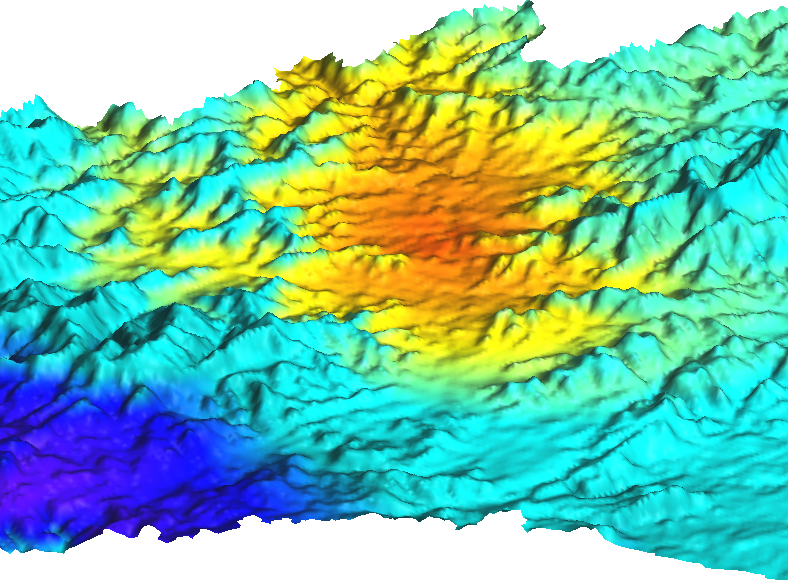
\includegraphics[width=\textwidth]{interpolation_precip_vvolrst}
Precipitation interpolated from meteorological stations in 3D space
using \gmodule{v.vol.rst} in the area of North Carolina mountains (USA)
\end{minipage}
~
\begin{minipage}{0.5\linewidth}
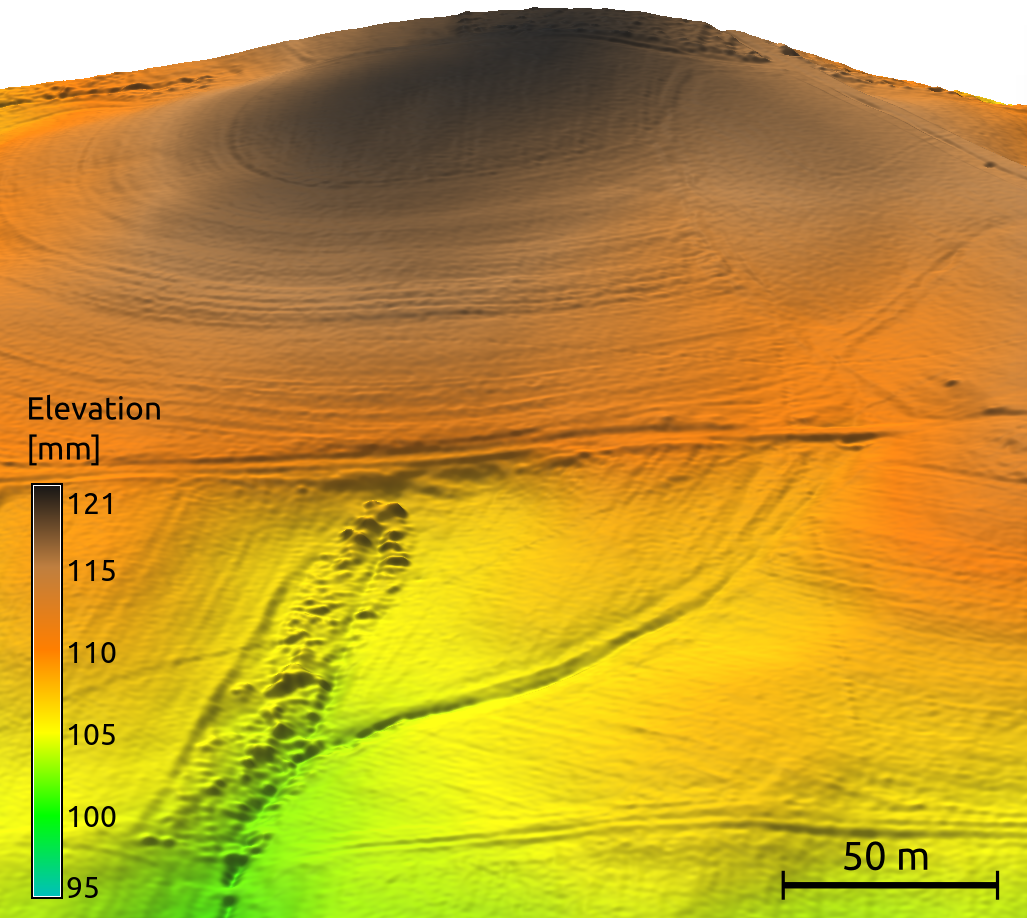
\includegraphics[width=\textwidth]{elevation_lidar}
Digital elevation model interpolated from LiDAR point clouds
using \gmodule{v.surf.rst}. Data are showing tillage in an agricultural field near Raleigh (North Carolina, USA)
\end{minipage}
}

%%%%%%%%%%%%%%%%%%%%%%%%%%%%%%%%%%%%%%%%%%%%%%%%%%%%%%%%%%%%%%%%%%%%%%%%%%%%%%%
\block{\blocktitlewrap{Evapotranspiration (ET)}}{
With the various types of actual ET models being developed in the last 20 years, 
it becomes necessary to inter-compare methods. Most already published ETa model 
comparisons address a low number of models, and small to medium areas 
(Chemin, 2014 \cite{chemin2012distributed}; Gao and Long, 2008 \cite{gao2008intercomparison}; 
Garcia et al., 2007 \cite{garcia2007comparison}; Suleiman et al., 2008
\cite{suleiman2008intercomparison}; Timmermans et al., 2007 \cite{timmermans2007intercomparison}). 
With the large amount of remote sensing data covering the Earth, and the daily 
information available for more than twelve years (i.e. Aqua/Terra-MODIS) for each pixel 
location, it becomes paramount to have a more complete comparison, 
in space and time.

\bigskip

\vspace*{1cm}

\begin{minipage}{0.5\linewidth}
\begin{center}
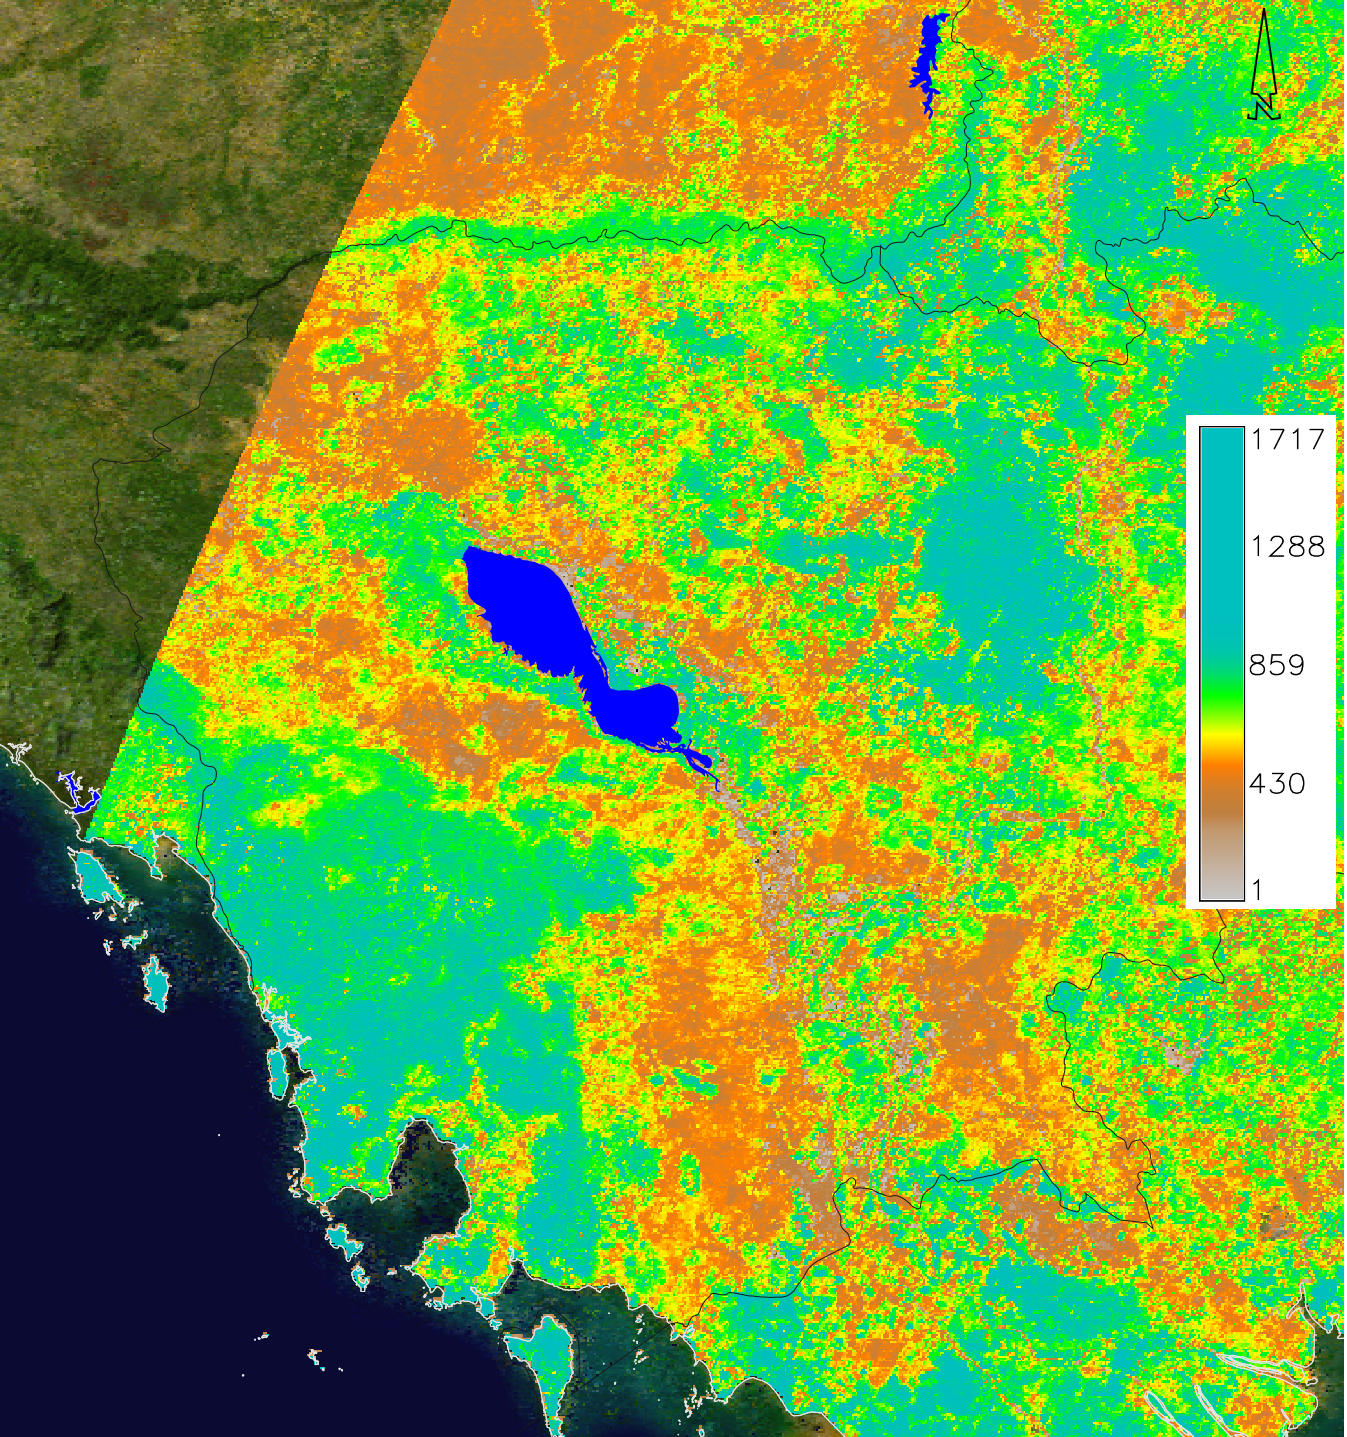
\includegraphics[width=0.9\textwidth]{TonleSapTa}
\end{center}
\end{minipage}
~
\begin{minipage}{0.5\linewidth}
\begin{center}
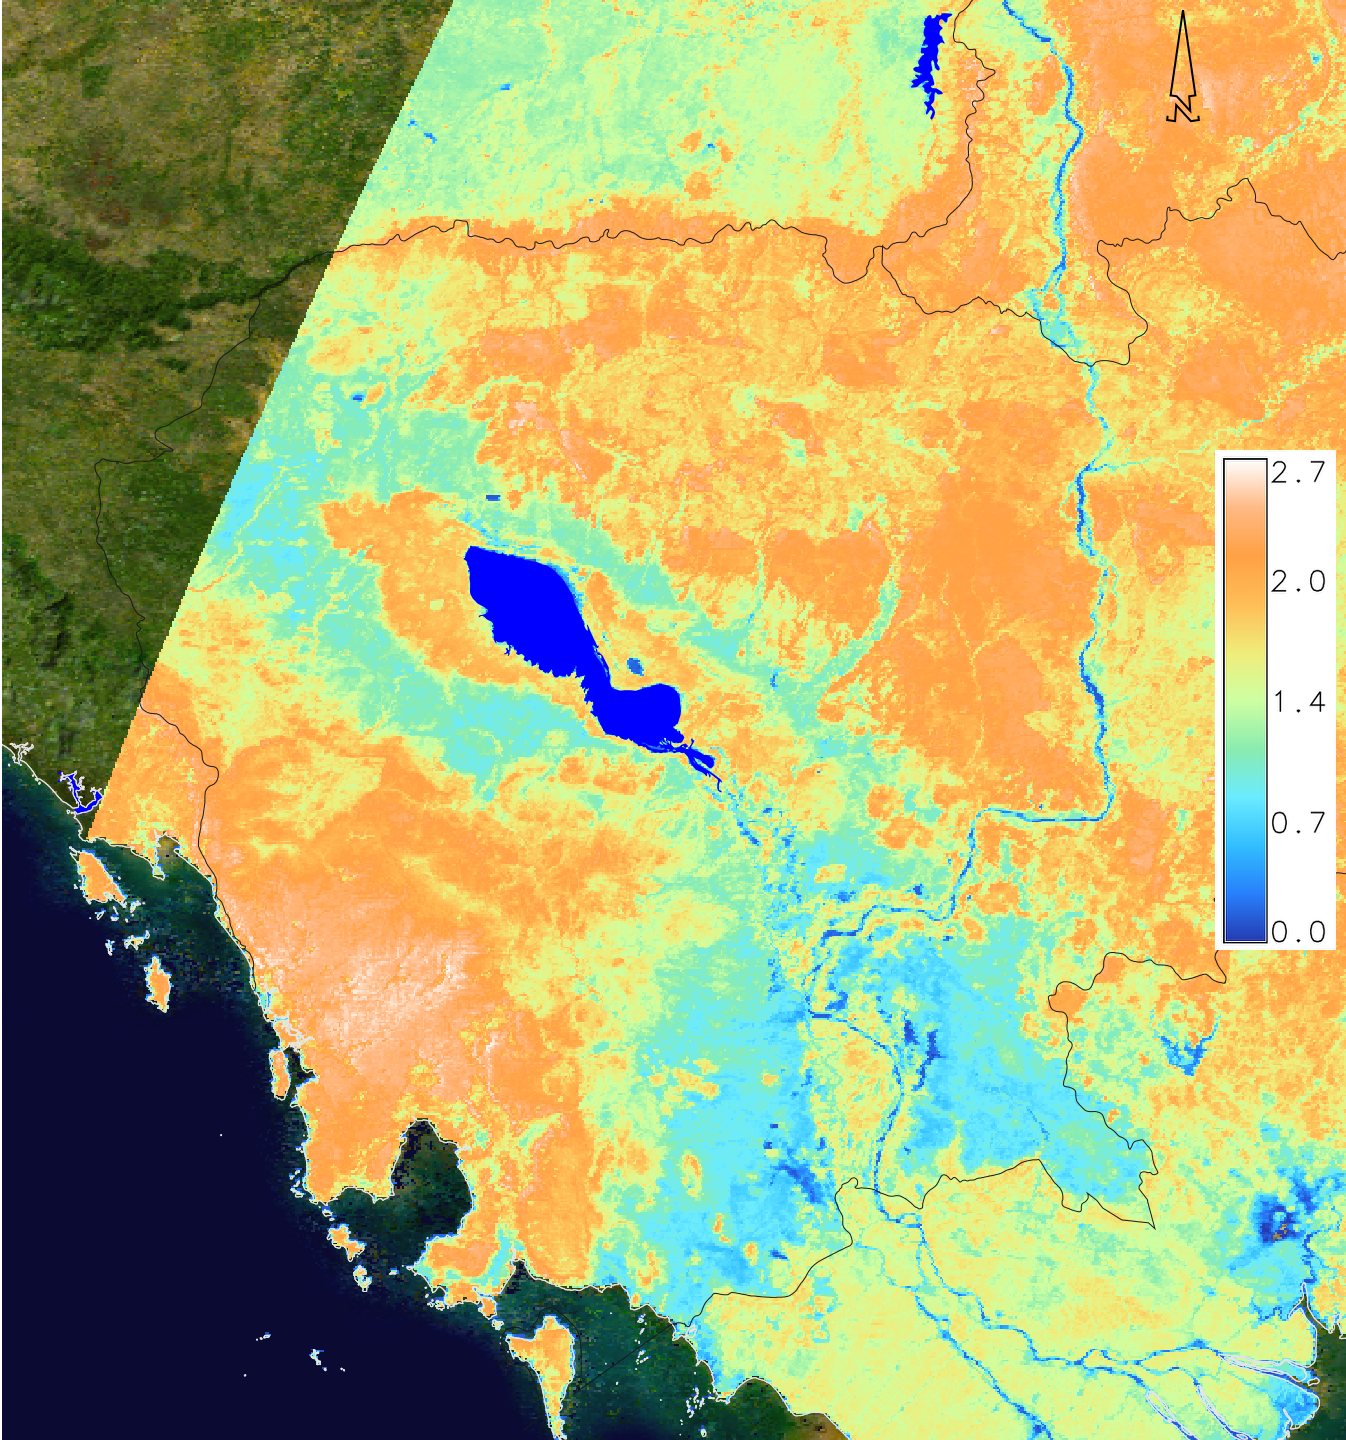
\includegraphics[width=0.9\textwidth]{TonleSapTaGap}
\end{center}
\end{minipage}
\vspace{2mm}
\begin{center}
Biological fraction of 2014 ET (cumul. mm/y) \& January average gap (mm/m), Tonle Sap, Cambodia.
\end{center}

\bigskip

To address this new experimental requirement, a distributed computing framework was 
designed and created (Chemin, 2012 \cite{chemin2012distributed}). 
The architecture design was built from original satellite datasets to various levels 
of processing until reaching the input dataset requirements of various ETa models. 
Each input product is computed once and reused in all ETa models requiring such input. 
This permits standardization of inputs as much as possible to reduce variations of 
models to their own internals/specificities. % can this sentence be rephrased 
All of the ET models are available in the 
new GRASS GIS version 7 as imagery modules and replicability is complete for future 
research.

\vspace*{0.6cm}

}


%%%%%%%%%%%%%%%%%%%%%%%%%%%%%%%%%%%%%%%%%%%%%%%%%%%%%%%%%%%%%%%%%%%%%
%%%%%%%%%%%%%%%%%%%%%%%%%%%%%%%%%%%%%%%%%%%%%%%%%%%%%%%%%%%%%%%%%%%%%
%%%%%%%%%%%%%%%%%%%%%%%%%%%%%%%%%%%%%%%%%%%%%%%%%%%%%%%%%%%%%%%%%%%%%
%%%%%%%%%%%%%%%%%%%%%%%%%%%%%%%%%%%%%%%%%%%%%%%%%%%%%%%%%%%%%%%%%%%%%
\column{0.25}

\block{\blocktitlewrap{Landscape structure}}{
A set of modules for multiscale analysis of landscape structure was added in 1992 
by Baker et al. \cite{baker1992r}, who developed the \gmodulenolink{r.le} model similar to 
FRAGSTATS \cite{mcgarigal1995fragstats}, see manual. The modules were gradually 
improved to become \gmodule{r.li} in 2006. Further development continued, with a significant 
increase in speed \cite{tracrli} and a new interactive user interface.
Rocchini et al. \cite{rocchini2013calculating} used \gmodule{r.li} modules to implement
high level tool for calculating landscape diversity.

\bigskip

\begin{minipage}{0.5\linewidth}
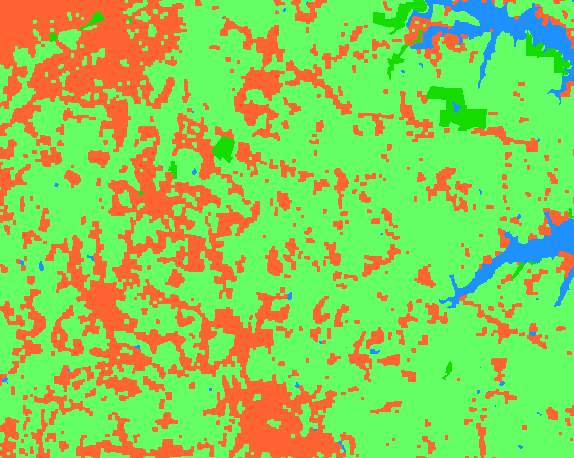
\includegraphics[width=\textwidth, trim={0 180 0 0}, clip]{diversity_classes}
\end{minipage}
\begin{minipage}{0.5\linewidth}
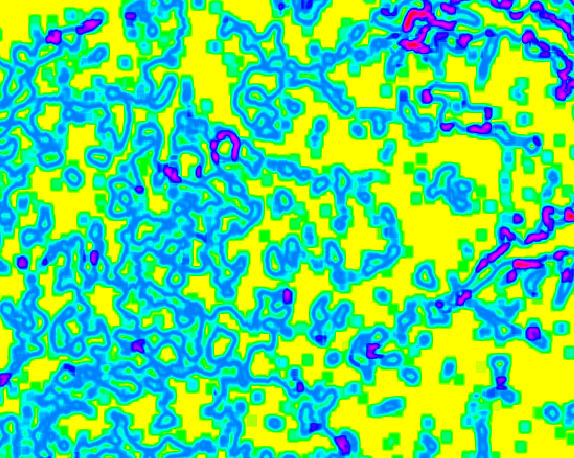
\includegraphics[width=\textwidth, trim={0 180 0 0}, clip]{diversity_shannon}
\end{minipage}

\medskip
Landuse classes and derived landscape diversity according to Shannon index in near Charlotte (NC, USA)
% r.diversity input=development_2006 prefix=diversity alpha=0.5 size=65
% r.li.shannon input="development_2006" config="conf_diversity_65.0" output="diversity_shannon_size_65.0"
}

%%%%%%%%%%%%%%%%%%%%%%%%%%%%%%%%%%%%%%%%%%%%%%%%%%%%%%%%%%%%%%%%%%%%%%%%%%%%%%%
\block{\blocktitlewrap{Conclusions}}{

\renewcommand{\labelitemi}{\textcolor{gray}{$\bullet$}\hspace{0.5ex}}

% TODO: review the points, it should be the highlight or something like that

\begin{itemize}
 \item Algorithms and models, included in GRASS GIS remain available long term (already for 30 years).
 \item The GRASS GIS development team takes care of API and operating system related changes. % in the provided contributions.
 \item Scientists can use highly specialized tools implemented by others as a result of having both scientific publications and source code at hand.
 \item The long term preservation of knowledge allows scientists to build new research and tools upon existing know-how.
\end{itemize}
}


%%%%%%%%%%%%%%%%%%%%%%%%%%%%%%%%%%%%%%%%%%%%%%%%%%%%%%%%%%%%%%%%%%%%%%%%%%%%%%%%
\block{\blocktitlewrap{References and Acknowledgements}}{

\vspace{-0.2cm}
\scriptsize

% \newcommand{\blocksectiontitle}[1]{\subsubsection*{\textcolor{gray}{\textsf{#1}}}}
\newcommand{\blocksectiontitle}[1]{\textbf{#1}}

%\blocksectiontitle{References}
\begingroup
\renewcommand{\section}[2]{}%
\bibliographystyle{plain}
\bibliography{poster}
\endgroup

\textcolor{gray}{
\hrulefill
}

\blocksectiontitle{Acknowledgements}

We acknowledge Matthew Horvath for \emph{Spill impacts from coal ash pond using GRASS GIS} and
% http://www4.ncsu.edu/~jcfounta/Summer14Posters/horvath.pdf
Eva Stopkova for physical model of High Tatras.

GRASS GIS project is a Open Source Geospatial Foundation (OSGeo) project and is using OSGeo infrastructure for Web site and code repository.

\vspace{-0.2cm}

\textcolor{gray}{
\hrulefill
}

\vspace{-0.1cm}

\newcommand{\qrcodesize}{0.05\linewidth}

% qrencode http://grass.osgeo.org -o qr_grass.eps -t EPS
% epspdf -b qr_grass.eps qr_grass.pdf

\begin{center}
\begin{tabular}{c}

% \hspace{5mm}

\begin{minipage}{\qrcodesize}

\includegraphics[width=\textwidth]{./images/qr_grass.pdf}
\end{minipage}
~
\begin{minipage}{0.15\linewidth}
\small {\href{http://grass.osgeo.org}{\nolinkurl{grass.osgeo.org}}}
\end{minipage}

\begin{minipage}{\qrcodesize}

\includegraphics[width=\textwidth]{./images/qr_grasswiki.pdf}
\end{minipage}
~
\begin{minipage}{0.2\linewidth}
\small {\href{http://grasswiki.osgeo.org}{\nolinkurl{grasswiki.osgeo.org}}}
\end{minipage}

\begin{minipage}{0.1\linewidth}
\href{http://creativecommons.org/licenses/by-sa/4.0/}{
\includegraphics[width=\textwidth]{ccbysa}}
\end{minipage}
~
\begin{minipage}{0.35\linewidth}
\small This poster is licensed under a Creative Commons Attribution-ShareAlike 4.0 International License.
\end{minipage}

\end{tabular}
\end{center}

\vspace{-0.08cm}
}

\end{columns}

\end{document}
